
\documentclass[12pt, a4paper, oneside, romanian]{teza-upb}
\setcounter{secnumdepth}{3}
\setcounter{tocdepth}{3}
\usepackage{babel}
\usepackage{graphicx}
\usepackage{adjustbox}
\usepackage{caption}
\usepackage{subcaption}
\usepackage{babel}
\usepackage{color}
\usepackage{graphicx}
\usepackage{ragged2e}
\usepackage{multirow}
\usepackage{amsmath}
\usepackage{mathtools}
\usepackage{enumitem}
\usepackage{float}
\usepackage{fontenc}
\usepackage{afterpage}
\usepackage{pdfpages}
\usepackage[
  bookmarks,
  bookmarksopen=true,
  pdftitle={Licenta},
  linktocpage]{hyperref}
\usepackage{url}

\singlespacing

%%%%%%%%%%%%%%%%%%%%%%%%%%%%%%%%%%%%%%%%%%%%%%%%%%%%%%%%cod colorat
\usepackage{listings}
\usepackage{color}
 
\definecolor{codegreen}{rgb}{0,0.6,0}
\definecolor{codegray}{rgb}{0.5,0.5,0.5}
\definecolor{codepurple}{rgb}{0.58,0,0.82}
\definecolor{backcolour}{rgb}{0.95,0.95,0.92
}
\DeclarePairedDelimiter\ceil{\lceil}{\rceil}

\newcommand\blankpage{%
    \null
    \thispagestyle{empty}%\
    \addtocounter{page}{-1}
    \newpage}

\lstdefinestyle{mystyle}{
	language=Matlab,
 %   backgroundcolor=\color{backcolour},   
    commentstyle=\color{codegreen},
    keywordstyle=\color{blue},
    numberstyle=\tiny\color{codegray},
    stringstyle=\color{codepurple},
	basicstyle=\ttfamily\scriptsize,
    breakatwhitespace=false,         
    breaklines=true,                 
    captionpos=b,                    
    keepspaces=true,                 
    numbers=left,                    
    numbersep=5pt,                  
    showspaces=false,                
    showstringspaces=false,
    showtabs=false,                  
    tabsize=2
}
 
\lstset{style=mystyle}
%%%%%%%%%%%%%%%%%%%%%%%%%%%%%%%%%%%%%%%%%%%%%%%

\begin{document}

\author{Stancovici Marian}

\title{Analiza imaginilor cu fund de ochi pentru ajutor în diagnosticul retinopatiei diabetice}


\facultatea{Facultatea de Electronică, Telecomunicații și Tehnologia Informației}
\tiplucrare{dizertație}
\domeniu{Calculatoare si Tehnologia Informatiei}
\catedra{Telecomunicații}
\campus{Leu}
\program{Ingineria Informaţiei}
\titlulobtinut{Master}
\director{Conf. dr. ing. Laura Maria FLOREA}

\submissionmonth{Iunie}
\submissionyear{2026}

\beforepreface

\newpage
\mbox{}
\newpage

\listoffigures

\listoftables

\newpage
\mbox{}
\newpage

\abbreviations{
  SOTA = State of the Art\\
  Deep DRiD = Deep Diabetic Retinopathy Image Dataset\\
  UoA-DR = University of Auckland Diabetic Retinopathy\\
  IDRiD = Indian Diabetic Retinopathy Image Dataset\\
  DDR = Dataset of Diabetic Retinopathy\\
  DRIVE = Digital Retinal Images for Vessel Extraction\\
}
%\preface{}
\afterpreface

\afterpage{\blankpage}

\chapter*{Introducere}

\section*{Contextul și motivația lucrării}

\ \ \ \ Retinopatia diabetică reprezintă o provocare majoră de sănătate publică, fiind principala cauză a
orbirii prevenibile în rândul populației active. Creșterea continuă a numărului de pacienți cu diabet
generează o presiune imensă asupra sistemelor medicale, depășind adesea capacitatea de screening a
specialiștilor. Deoarece afecțiunea poate evolua asimptomatic în fazele inițiale, identificarea pacienților
la risc este critică înainte ca leziunile retiniene să devină ireversibile, subliniind necesitatea unor soluții
de monitorizare scalabile și eficiente.
\bigskip

Complexitatea diagnosticării este dată de necesitatea unei clasificări precise, conform
standardelor internaționale care împart boala în cinci clase de severitate \cite{6_wang2021deep}, \cite{11_shakibania2024dual}. Procesul impune
medicului să distingă între stadiile incipiente, marcate doar de microanevrisme discrete \cite{13_staal2004ridge}, și formele
avansate, caracterizate de hemoragii și neovascularizație. Această granularitate a diagnosticului este
dificilă de menținut constant în programele de screening în masă, unde oboseala și subiectivitatea
factorului uman pot duce la erori de clasificare cu impact direct asupra deciziilor terapeutice.
\bigskip

Pentru a depăși aceste limitări, domeniul imagisticii medicale a adoptat rapid soluțiile bazate pe
inteligență artificială. Trecerea de la metodele clasice de procesare a imaginii \cite{2_sopharak2009automatic} la algoritmii de învățare
profundă (Deep Learning) a marcat un punct de inflexiune, validat clinic prin studii extensive \cite{3_gulshan2016development}. Rețelele
neurale convoluționale au eliminat necesitatea definisrii manuale a regulilor vizuale \cite{4_pratt2016convolutional}, având capacitatea
de a învăța autonom trăsături complexe direct din datele brute \cite{9_chetoui2020explainable} și de a identifica corelații subtile între
texturi și patologie.
\bigskip

Evoluția recentă a acestor tehnologii a permis tranziția de la modele experimentale simple la
arhitecturi robuste \cite{7_huang2022rtnet}, capabile să opereze în condiții clinice reale. Cercetarea actuală s-a distanțat de
clasificarea binară elementară, concentrându-se pe sisteme care pot gestiona variabilitatea imaginilor
provenite din diverse surse prin tehnici de adaptare la domeniu \cite{8_zhang2022multi}. Algoritmii moderni demonstrează o
reziliență crescută la artefacte și zgomot vizual, oferind o consistență a diagnosticului care rivalizează cu
expertiza umană \cite{9_chetoui2020explainable}, \cite{10_jabbar2022transfer}.

\section*{Obiectivele lucrării}

\ \ \ \ Scopul lucrării de față este de a folosi algoritmi de vedere computerizată bazați pe rețele convoluționale adânci pentru a crea o metodă de detectare
si clasificare a retinopatiei diabetice. Metoda se va testa pe seturi de date publice. Implementarea se va face în Python folosind biblioteci specifice.
\bigskip

Aceasta urmărește atingerea următoarelor obiective:

\begin{itemize}
  \item Analizarea metodelor deja propuse în literatura de specialitate pentru detecția și clasificarea automată a retinopatiei diabetice folosind 
  imagini cu fund de ochi.

  \item Căutarea seturilor de date publice ce conțin imagini cu fund de ochi și adnotări pentru clasificarea retinopatiei diabetice.

  \item Analizarea seturilor de date găsite.

  \item Propunerea unei metode bazate pe învățare profundă pentru detecția și clasificarea retinopatiei diabetice.

  \item Analizarea performanței pentru metoda propusă în diverse cazuri de antrenare/testare
\end{itemize}

\section*{Structura lucrării}

Lucrarea de față este structurată în mai multe capitole, fiecare din ele abordând un subiect esențial din proiect:

\begin{itemize}
  \item Capitolul 1: Introducere
        \begin{itemize}[label={}]
          \item În acest capitol se prezintă contextul și motivația lucrării, cât și cum se propune să se redacteze si să se structureze, menționând aplicabilitatea acesteia in lumea reală.
        \end{itemize}

  \item Capitolul 2: Fundamente teoretice - context medical și tehnic
        \begin{itemize}[label={}]
          \item[] Acest capitol va oferi o privire de ansamblu asupra retinopatiei diabetice, explicând cauzele, simptomele și stadiile acestei afecțiuni, precum și importanța detecției și clasificării automate a acesteia. De asemenea, se vor introduce conceptele de bază ale învățării profunde și ale rețelelor neuronale convoluționale, care vor fi utilizate în dezvoltarea metodei propuse.
        \end{itemize}

  \item Capitolul 3: Metode existente pentru detecția automată a retinopatiei diabetice
        \begin{itemize}[label={}]
          \item[] Acest capitol va oferi o analiză detaliată a metodelor existente pentru detecția și clasificarea retinopatiei diabetice, evidențiind avantajele și limitările acestora, precum și modul în care acestea au evoluat în timp.
        \end{itemize}

  \item Capitolul 4: Metodologie și implementare
        \begin{itemize}[label={}]
          \item[] Acest capitol va detalia metodologia și implementarea propusă pentru detecția și clasificarea retinopatiei diabetice, explicând arhitectura rețelei neuronale utilizate, procesul de antrenare și optimizare, precum și modul în care aceasta se diferențiază de metodele existente.
        \end{itemize}

  \item Capitolul 5: Metoda propusă
        \begin{itemize}[label={}]
          \item[] Acest capitol va detalia metoda propusă pentru detecția și clasificarea retinopatiei diabetice, explicând arhitectura rețelei neuronale utilizate, procesul de antrenare și optimizare, precum și modul în care aceasta se diferențiază de metodele existente.
        \end{itemize}

  \item Capitolul 6: Rezultate experimentale și discuții
        \begin{itemize}[label={}]
          \item[] Acest capitol va prezenta rezultatele obținute în urma testării metodei propuse pe seturile de date alese, comparând performanța acesteia cu alte metode existente și discutând avantajele și limitările sale.
        \end{itemize}

  \item Capitolul 7: Concluzii
        \begin{itemize}[label={}]
          \item[] Acest capitol va sintetiza concluziile generale ale lucrării, evidențiind contribuțiile aduse și impactul potențial al metodei propuse în domeniul detecției automate a retinopatiei diabetice.
        \end{itemize}
\end{itemize}

\newpage
\mbox{}
\newpage


\chapter{Fundamente teoretice - context medical și tehnic}

\section{Diabetul zaharat și complicațiile sale oculare}

\section{Anatomia ochiului și retina}

\section{Retinopatia diabetică — definiție, stadii de evoluție și simptome}

\section{Imagistica de fund de ochi ("fundus photography")}

\section{Diagnosticul clinic — procesul actual și limitările sale}


\chapter{Metode existente pentru detecția automată a retinopatiei diabetice}

\section{Analiza seturilor de date disponibile}

\ \ \ \ Performanța și capacitatea de generalizare a modelelor de învățare profundă sunt intrinsec
dependente de calitatea, volumul și diversitatea datelor utilizate în procesul de antrenare. În contextul
oftalmologiei computaționale, disponibilitatea bazelor de date publice a permis tranziția de la metodele
clasice de procesare a imaginii la arhitecturi neuronale complexe, oferind un teren comun pentru
evaluarea obiectivă a algoritmilor.

\begin{itemize}
  \item \textbf{Seturi de referință pentru clasificarea globală (“Grading”)}
  
      \begin{itemize}
          \item \textbf{EyePACS} (Kaggle Diabetic Retinopathy Detection) \cite{3_gulshan2016development}, \cite{9_chetoui2020explainable} rămâne cea mai 
                vastă resursă publică disponibilă, conținând aproximativ 88.702 de imagini. Importanța sa strategică constă în eterogenitatea
                extremă a imaginilor (variații de expunere, focalizare, artefacte), fiind critic pentru antrenarea unor
                rețele backbone robuste capabile să gestioneze fenomenul de “domain shift” \cite{8_zhang2022multi} și să generalizeze pe
                imagini de calitate slabă

          \item \textbf{APTOS 2019} Blindness Detection \cite{9_chetoui2020explainable} reprezintă standardul modern de calitate. Colectat de Aravind Eye
                Hospital, acest set de 3.662 de imagini este utilizat frecvent în literatura recentă pentru “fine-tuning”,
                oferind o vizibilitate superioară a detaliilor retiniene comparativ cu seturile mai vechi

          \item \textbf{MESSIDOR-2} \cite{9_chetoui2020explainable} este considerat în prezent „Benchmark-ul de Aur” pentru testarea algoritmilor.
                Extinzând setul original Messidor la 1.748 de imagini, acesta se distinge prin consistența diagnostică și
                este utilizat ca domeniu țintă (Target Domain) în studiile de adaptare \cite{8_zhang2022multi} și pentru validarea sistemelor
                explicabile (XAI) \cite{9_chetoui2020explainable}, oferind o metrică fidelă a performanței reale pe date curate.

          \item \textbf{DeepDRiD} \cite{14_liu2022deepdrid} aduce o inovație necesară prin structurarea
                celor 2.000 de imagini în perechi binoculare și includerea notelor de calitate, simulând fluxul de triaj
                clinic.

          \item \textbf{UoA-DR} \cite{9_chetoui2020explainable} este o resursă istorică (~200 imagini), utilizată
                complementar în studiile comparative pentru a asigura diversitatea demografică a validării.
      \end{itemize}

  \item \textbf{Seturi specializate pentru segmentarea leziunilor și analiza detaliată}

      \begin{itemize}
        \item \textbf{IDRiD} \cite{9_chetoui2020explainable} este setul critic pentru sarcinile de segmentare
              semantică fină \cite{7_huang2022rtnet}. Pentru 81 dintre imagini, experții au trasat manual măști binare la nivel de pixel,
              făcându-l indispensabil pentru antrenarea arhitecturilor complexe de tip Transformer și pentru validarea
              localizării leziunilor în sistemele end-to-end \cite{9_chetoui2020explainable}.

        \item \textbf{DDR} \cite{15_li2019diagnostic} a revoluționat segmentarea pe scară largă, oferind 13.673 de
              imagini. Este esențial pentru antrenarea rețelelor adânci de segmentare (precum RTNet) fără a risca
              “overfitting-ul”, oferind adnotări “pixel-wise” pentru leziuni multiple \cite{7_huang2022rtnet}.

        \item \textbf{E-Ophtha} \cite{9_chetoui2020explainable} este o bază de date vitală pentru reducerea alarmelor false în metodele de detecție a
              exudatelor \cite{2_sopharak2009automatic}. Valoarea sa unică constă în includerea imaginilor cu patologii non-diabetice care pot fi
              confundate cu DR

        \item DiaRetDB1 \cite{9_chetoui2020explainable} este standardul istoric pentru calibrarea sensibilității la leziuni roșii (microanevrisme) în
              lucrările de detecție automată \cite{1_niemeijer2005automatic}. Complementar, HEI-MED \cite{16_giancardo2012exudate} oferă 169 de imagini focalizate exclusiv
              pe segmentarea zonelor de Edem Macular Diabetic.

        \begin{figure}[h]
        \centering
        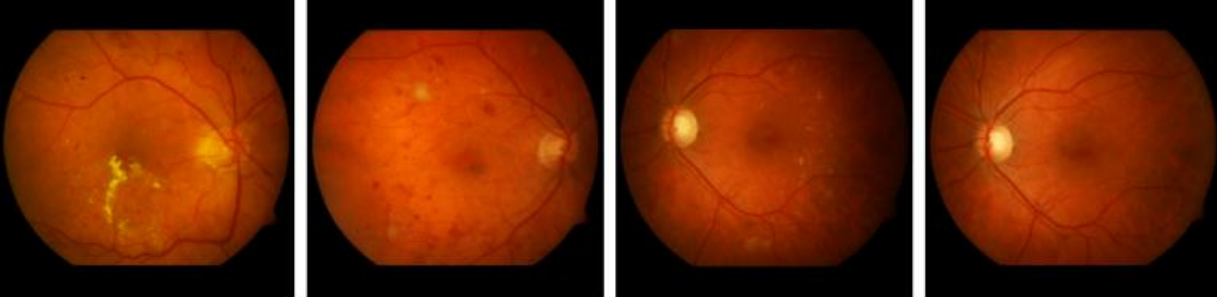
\includegraphics[width=1\columnwidth]{Figuri/Fig1_Eye-fundus-examples.png}
        \captionsetup{justification=centering}
        \caption{Exemple de imagini ale fundului de ochi în seturile de date DIARETDB0 și DIARETDB1 \cite{9_chetoui2020explainable}}
        \label{fig: Examples-fundus-eyes}
        \end{figure}

      \end{itemize}

  \item \textbf{Seturi standard pentru preprocesarea vasculară}
  
        \begin{itemize}
          \item \textbf{DRIVE} \cite{13_staal2004ridge} și STARE \cite{9_chetoui2020explainable} sunt pilonii etapei de preprocesare.
                Deși conțin un număr redus de imagini, ele sunt utilizate obligatoriu pentru validarea algoritmilor de
                segmentare a vaselor de sânge, cum ar fi arhitecturile U-Net modificate \cite{12_sambyal2020modified} sau metodele clasice de
                extragere a trăsăturilor \cite{1_niemeijer2005automatic}.

                Tabelul de mai jos sintetizează caracteristicile tehnice esențiale ale seturilor de date analizate,
                evidențiind diferențele de volum, rezoluție și tipul de adnotare disponibil, elemente care dictează
                utilizarea lor în diversele etape ale proiectului.

            \begin{figure}[h]
            \centering
            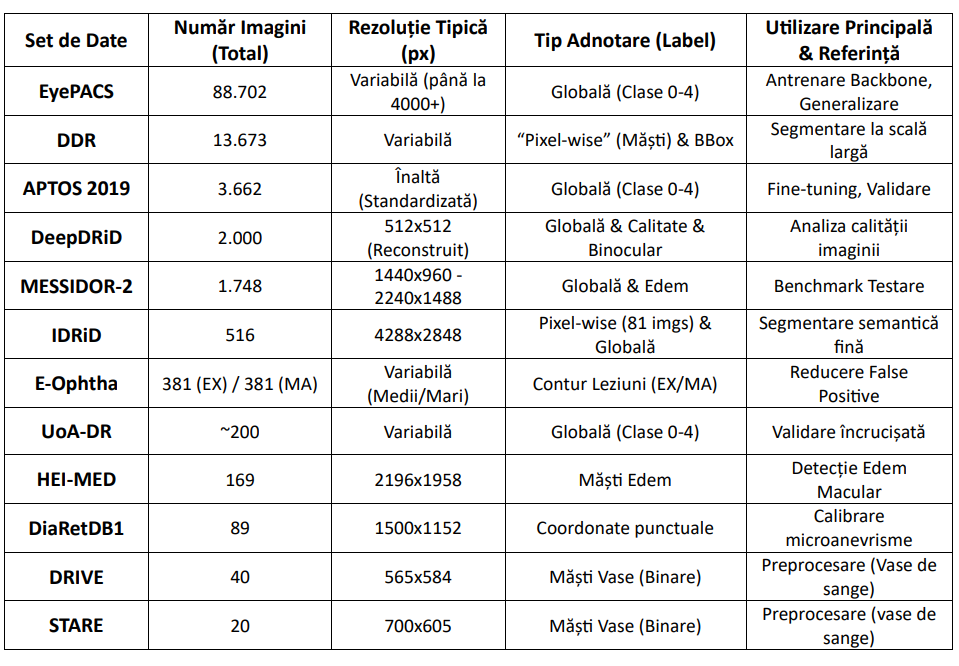
\includegraphics[width=0.75\columnwidth]{Figuri/Tabel1_Datasets_diff.png}
            \caption{Tabel comparativ intre seturile de date disponibile}
            \label{fig: table-datasets}
            \end{figure}

        \end{itemize}
\end{itemize}

\section{Metoda bazată pe arhitectura Inception-V3 \cite{3_gulshan2016development}}

\ \ \ \ Studiul realizat de Gulshan et al. \cite{3_gulshan2016development} este considerat un reper major în literatura de specialitate,
marcând una dintre primele validări clinice riguroase ale utilizării rețelelor neuronale convoluționale
pentru screening-ul automat al retinopatiei diabetice. Lucrarea demonstrează că un sistem de deep
learning poate atinge și chiar depăși performanța medie a medicilor oftalmologi în detectarea
retinopatiei diabetice, contribuind decisiv la acceptarea inteligenței artificiale în aplicații medicale reale
\cite{3_gulshan2016development}.
\bigskip

Arhitectura utilizată este Inception-v3, o rețea convoluțională profundă caracterizată prin
utilizarea modulelor Inception, care combină în paralel convoluții de dimensiuni diferite (1×1, 3×3, 5×5)
și operații de pooling. Această strategie permite captarea informațiilor la multiple scări spațiale și reduce
costul computațional prin utilizarea convoluțiilor 1×1 pentru diminuarea dimensionalității. Datorită
acestei structuri, modelul este capabil să învețe reprezentări vizuale complexe, esențiale pentru
identificarea leziunilor subtile specifice retinopatiei diabetice.
\bigskip

Modelul a fost antrenat pe un set de date extins, alcătuit din peste 128.000 de imagini fundus
color, etichetate independent de mai mulți medici oftalmologi certificați în 2015. Utilizarea consensului
între experți a contribuit la reducerea subiectivității etichetelor și la creșterea fiabilității procesului de
antrenare. Sarcina principală a rețelei a fost clasificarea imaginilor în funcție de prezența sau absența
retinopatiei diabetice referabile, conform standardelor clinice acceptate internațional \cite{3_gulshan2016development}.
\bigskip

Preprocesarea imaginilor a inclus decuparea automată a regiunii retiniene, redimensionarea la o
rezoluție compatibilă cu Inception-v3 și normalizarea intensității pixelilor. În plus, au fost aplicate tehnici
extensive de augmentare a datelor, precum rotații, translații și ajustări de luminozitate și contrast, pentru
a îmbunătăți generalizarea și a reduce supraînvățarea \cite{3_gulshan2016development} \cite{10_jabbar2022transfer}.
\bigskip

Evaluarea performanței a fost realizată pe seturile de date EyePACS-1 și Messidor-2 \cite{9_chetoui2020explainable}, unde modelul a
obținut o arie sub curba ROC (AUC) de aproximativ 0.99 pentru detectarea retinopatiei diabetice
referabile, cu valori ridicate de sensibilitate, comparabile cu performanța medicilor oftalmologi
experimentați \cite{3_gulshan2016development} \cite{4_pratt2016convolutional}.

\section{“Transfer Learning” pentru diagnosticul retinopatiei diabetice \cite{10_jabbar2022transfer}}

\ \ \ \ Lucrarea propusă de Jabbar et al. \cite{10_jabbar2022transfer} abordează problema diagnosticului automat al
retinopatiei diabetice dintr-o perspectivă practică, concentrându-se pe utilizarea tehnicilor de “transfer
learning” pentru a compensa limitările impuse de dimensiunea redusă a seturilor de date medicale
etichetate. Studiul evidențiază faptul că modelele CNN pre-antrenate pe seturi de date generale de mari
dimensiuni, precum ImageNet, pot fi adaptate eficient pentru analiza imaginilor fundus, obținând
performanțe competitive cu un cost de antrenare semnificativ redus \cite{10_jabbar2022transfer}.
\bigskip

Autorii investighează mai multe arhitecturi consacrate de rețele neuronale convoluționale,
printre care VGG16, VGG19, ResNet50, Inception-v3 și DenseNet, utilizate ca extractoare de
caracteristici. Strategia de transfer learning constă în inițializarea rețelelor cu ponderi pre-antrenate,
urmată de ajustarea straturilor superioare pentru sarcina specifică de clasificare a retinopatiei diabetice.
În unele experimente, straturile convoluționale inferioare sunt înghețate pentru a preveni
supraînvățarea, în timp ce în altele este aplicat “fine-tuning” progresiv pentru a îmbunătăți adaptarea la
domeniul imagisticii medicale. Una din abordările propuse poate fi observată în figura următoare.

\begin{figure}[h]
\centering
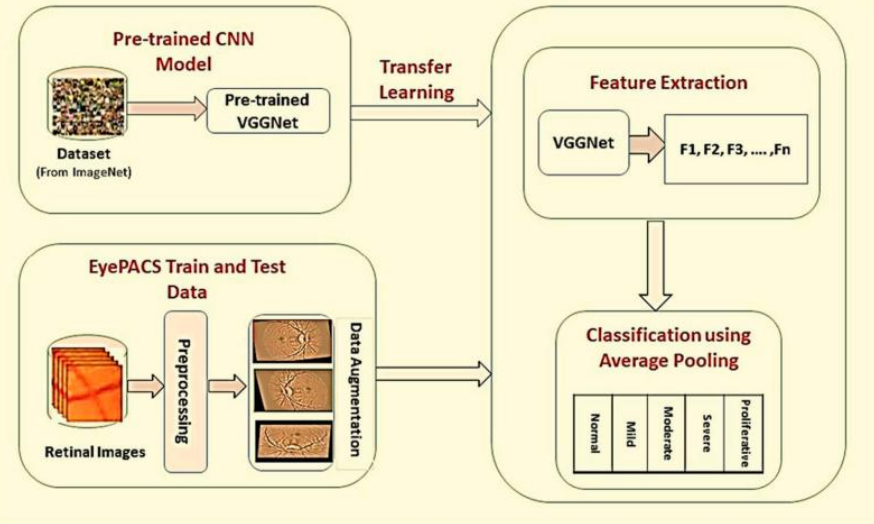
\includegraphics[width=1\columnwidth]{Figuri/Recommended_framework.png}
\captionsetup{justification=centering}
\caption{Framework propus pentru detectarea și clasificarea retinopatiei diabetice \cite{10_jabbar2022transfer}}
\label{fig: recommended-framework}
\end{figure}

\bigskip

Seturile de date utilizate includ imagini fundus publice din Kaggle EyePACS \cite{9_chetoui2020explainable}, preprocesate prin
redimensionare, normalizare și augmentare extensivă a datelor. Tehnicile de augmentare, precum
rotațiile, flip-urile orizontale și ajustările de luminozitate, joacă un rol central în creșterea diversității
artificiale a datelor și în îmbunătățirea capacității de generalizare a modelelor. Această etapă este
esențială în contextul “transfer learning-ului”, unde diferențele de distribuție dintre datele naturale și
imaginile medicale pot afecta performanța rețelelor \cite{10_jabbar2022transfer}.
\bigskip

Evaluarea performanței este realizată folosind metrici standard, precum acuratețea,
sensibilitatea, specificitatea și scorul F1, permițând o comparație riguroasă între diferitele arhitecturi
analizate. Rezultatele experimentale indică faptul că modelele bazate pe DenseNet și ResNet obțin
performanțe superioare față de arhitecturile mai vechi, confirmând avantajele reutilizării caracteristicilor
vizuale generale în sarcini medicale specializate. Studiul subliniază că transfer learning-ul reprezintă o
soluție viabilă și eficientă pentru implementarea rapidă a sistemelor automate de screening în contexte
cu resurse limitate \cite{10_jabbar2022transfer}.

\section{“Multi-task Learning” pentru gradarea retinopatiei diabetice \cite{6_wang2021deep}}

\ \ \ \ Lucrarea propusă de Wang et al. \cite{6_wang2021deep} introduce o abordare de tip “deep multi-task learning”
pentru gradarea automată a retinopatiei diabetice, având ca obiectiv principal exploatarea relației clinice
dintre severitatea bolii și prezența leziunilor retiniene specifice. Spre deosebire de metodele clasice de
clasificare “single-task”, autorii demonstrează că învățarea simultană a mai multor sarcini corelate clinic
conduce la reprezentări vizuale mai discriminative și la performanțe superioare în sarcina principală de
gradare \cite{6_wang2021deep}.
\bigskip

Arhitectura propusă este alcătuită dintr-un backbone convoluțional comun, bazat pe o rețea CNN
profundă (ResNet18), utilizat pentru extracția caracteristicilor globale din imaginile fundus. Peste acest
extractor comun sunt construite mai multe ramuri specializate (task-specific branches), fiecare 
corespunzătoare unei sarcini distincte. Sarcina principală constă în clasificarea severității retinopatiei
diabetice în mai multe stadii, în timp ce sarcinile auxiliare vizează detectarea prezenței diferitelor tipuri
de leziuni, precum microanevrismele, exudatele dure, exudatele moi și hemoragiile, considerate
“markeri” clinici relevanți ai progresiei bolii \cite{6_wang2021deep}.
\bigskip

Un element central al arhitecturii îl reprezintă mecanismul de partajare controlată a
caracteristicilor între sarcini. În locul unei separări rigide între ramuri, modelul permite propagarea
informației relevante între sarcina de gradare și cele de detecție a leziunilor, încurajând învățarea unor
reprezentări comune sensibile la semnalele patologice fine. Funcția de pierdere globală este definită ca o
combinație ponderată a pierderilor individuale asociate fiecărei sarcini:

$$L_{isr} = \lambda_{img} \cdot L_{img\_isr} + \lambda_{tv} \cdot L_{tv\_isr} + \lambda_{sa} \cdot L_{seg\text{-}aware} + \lambda_{ca} \cdot L_{cls\text{-}aware}$$
\bigskip

,unde $\lambda_{img}$, $\lambda_{tv}$, $\lambda_{sa}$ și $\lambda_{ca}$ sunt hiperparametri care controlează 
contribuția pierderilor ``intra-task'', ``segmentation-aware'' și ``classification-aware''. Această formulare permite echilibrarea
influenței fiecărei sarcini și stabilizează procesul de optimizare \cite{6_wang2021deep}.

Modelul este antrenat și evaluat pe seturi de date publice de imagini fundus etichetate (DDR
\cite{15_li2019diagnostic} si EyePACS \cite{9_chetoui2020explainable}) atât cu stadiul retinopatiei diabetice, cât și cu adnotări la nivel de imagine privind
prezența leziunilor. Imaginile sunt supuse unor etape standard de preprocesare, incluzând decuparea
regiunii retiniene, redimensionarea și augmentarea datelor, pentru a reduce variațiile de iluminare și
pentru a îmbunătăți capacitatea de generalizare. Prin includerea sarcinilor auxiliare, modelul beneficiază
de un efect de regularizare implicită, reducând riscul de supraînvățare, aspect observat și în lucrările
anterioare bazate pe CNN-uri “single-task” \cite{3_gulshan2016development}, \cite{4_pratt2016convolutional}.
\bigskip

Rezultatele experimentale raportate în articol indică îmbunătățiri consistente ale performanței
față de modelele “single-task”, atât în termeni de acuratețe, cât și de scor F1 pentru sarcina de gradare a
retinopatiei diabetice. În plus, autorii evidențiază o creștere a stabilității predicțiilor și o sensibilitate mai
bună la stadiile intermediare ale bolii, considerate dificil de clasificat. Aceste rezultate confirmă faptul că
integrarea informațiilor despre leziuni în procesul de antrenare contribuie direct la o evaluare mai
precisă a severității retinopatiei diabetice și validează eficiența paradigmei “multi-task learning” în
context clinic \cite{6_wang2021deep}.
\bigskip

\section{Analiza arhitecturii “Modified U-Net” pentru segmentarea semantică \cite{12_sambyal2020modified}}

\ \ \ \ Segmentarea semantică a structurilor retiniene, în special a rețelei vasculare și a leziunilor
asociate retinopatiei diabetice, reprezintă o etapă critică în diagnosticarea automată, deoarece
modificările morfologice ale vaselor de sânge sunt adesea primii indicatori ai bolii. Deși arhitectura UNet, introdusă inițial de Ronneberger 
et al. \cite{5_ronneberger2015u} pentru segmentarea biomedicală, a devenit standardul de
aur în domeniu datorită structurii sale simetrice de tip “encoder-decoder”, aceasta prezintă limitări în
detectarea vaselor capilare foarte fine, pierzând informații spațiale esențiale în procesul de subeșantionare.
\bigskip

În studiul "Modified U-Net architecture for semantic segmentation of diabetic retinopathy
images", Sambyal et al \cite{12_sambyal2020modified}. propun o optimizare arhitecturală semnificativă pentru a contracara aceste
deficiențe. Modelul propus, denumit Modified U-Net, păstrează structura în formă de „U” a rețelei
originale, dar inovează fundamental la nivelul blocurilor de procesare.
\bigskip

Autorii au înlocuit blocurile convoluționale standard cu blocuri reziduale (residual blocks),
inspirate din arhitecturile de tip ResNet. Această modificare este crucială din punct de vedere tehnic: în
rețelele adânci, apare frecvent problema dispariției gradientului (vanishing gradient), ceea ce face
antrenarea dificilă și duce la pierderea detaliilor fine. Prin introducerea conexiunilor reziduale (“skip
connections” la nivel de bloc), informația originală este propagată mai eficient prin straturi, permițând
rețelei să învețe caracteristici complexe fără a degrada performanța pe detaliile de finețe, precum
microanevrismele sau vasele subțiri. Aceste detalii se pot observa și în figura următoare.

\begin{figure}[h]
\centering
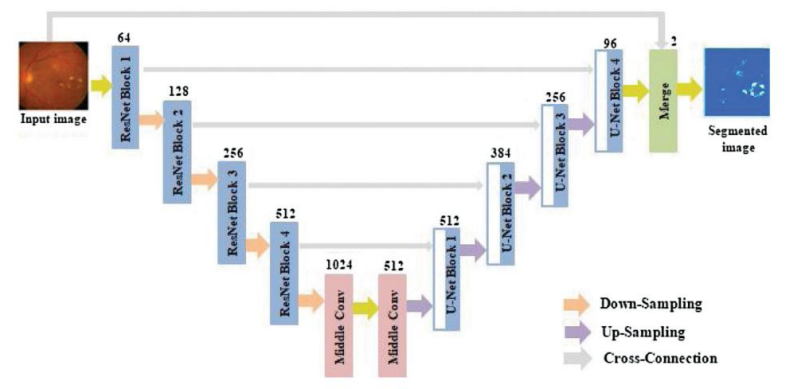
\includegraphics[width=1\columnwidth]{Figuri/modified-u-net.png}
\captionsetup{justification=centering}
\caption{Arhitectura U-net modificată \cite{12_sambyal2020modified}}
\label{fig: modified-u-net}
\end{figure}

\bigskip

Importanța acestei abordări constă în capacitatea de generalizare comparativ cu metodele
clasice de procesare a imaginii, precum cele bazate pe “clustering fuzzy” propuse anterior de Sopharak et
al. \cite{2_sopharak2009automatic}. În timp ce metodele de tip “clustering” sunt sensibile la zgomot și la variațiile de iluminare
(frecvente în imaginile de fund de ochi), arhitectura Modified U-Net demonstrează o robustețe sporită
prin învățarea contextuală a trăsăturilor
\bigskip

Pentru validarea performanței, metoda a fost testată pe seturile de date publice standardizate
DRIVE \cite{13_staal2004ridge} și STARE \cite{9_chetoui2020explainable}, recunoscute pentru dificultatea lor în segmentarea vaselor.

Rezultatele experimentale raportate de Sambyal et al. \cite{12_sambyal2020modified} au indicat o îmbunătățire clară față de
U-Net-ul standard. Pe setul de date DRIVE, autorii au obținut o acuratețe maximă de 96.94% și o arie de
sub curba ROC (AUC) de 0.98, valori care plasează metoda în topul soluțiilor de segmentare. Mai mult,
analiza vizuală a rezultatelor arată o continuitate mult mai bună a vaselor de sânge segmentate și o
reducere a alarmelor false în zonele cu patologii, demonstrând că integrarea învățării reziduale în
arhitectura de segmentare este o direcție esențială pentru analiza detaliată a retinopatiei diabetice.

\section{Tranziția către arhitecturi globale: RTNet (Relation Transformer Network) \cite{7_huang2022rtnet}}

\ \ \ \ Dacă modelele bazate pe U-Net, precum cel discutat anterior \cite{12_sambyal2020modified}, excelează în capturarea
detaliilor locale, ele suferă totuși de o limitare inerentă a rețelelor convoluționale: incapacitatea de a
modela dependențe la distanță mare (long-range dependencies). În patologia retiniană, leziunile nu apar
izolat; există adesea o corelație spațială între poziția vaselor de sânge și apariția microanevrismelor sau a
exudatelor. Pentru a adresa această lipsă de „context global”, Huang et al. \cite{7_huang2022rtnet} au propus în 2022 o
schimbare de paradigmă prin introducerea RTNet (Relation Transformer Network), o arhitectură care
marchează trecerea către mecanismele de atenție.
\bigskip

Inovația centrală a RTNet constă în înlocuirea parțială a operațiilor convoluționale standard cu
blocuri de tip “Transformer”, denumite Relation Transformer Blocks (RTB). Spre deosebire de CNN-uri
care „văd” doar o fereastră mică de pixeli la un moment dat, RTB-ul utilizează două mecanisme de
atenție complementare:

\begin{enumerate}
  \item “Self-Attention” (Atenție proprie): Permite modelului să înțeleagă relațiile dintre leziunile
        dispersate pe toată suprafața retinei (de exemplu, grupuri de exudate dure care semnalează o
        zonă de edem).

\item “Cross-Attention” (Atenție încrucișată): Autorii au observat că leziunile vasculare sunt strâns
      legate de structura vaselor de sânge. Astfel, mecanismul de “cross-attention” folosește harta
      vaselor de sânge ca un „ghid” pentru a localiza mai precis leziunile fine, transferând informație
      structurală dinspre ramura vasculară către ramura de detectare a leziunilor.
\end{enumerate}
\bigskip

Pentru validare, metoda a fost testată pe seturile de date IDRiD \cite{9_chetoui2020explainable} și DDR \cite{15_li2019diagnostic}, care conțin adnotări
la nivel de pixel pentru multiple tipuri de leziuni. Rezultatele cantitative au demonstrat că RTNet
depășește metodele existente anterioare (inclusiv diverse variante de U-Net și DeepLab), obținând cele
mai bune scoruri de segmentare pentru Exudate (EX), Microanevrisme (MA) și Exudate Moi (SE).
\bigskip

Deși inovația teoretică a arhitecturii RTNet (Relation Transformer Network) propusă de Huang et al.
\cite{7_huang2022rtnet} este evidentă prin integrarea mecanismelor de atenție, validarea practică a acesteia necesită o
demonstrație riguroasă a faptului că fiecare modul propus contribuie activ la îmbunătățirea segmentării.
În acest sens, autorii au realizat un studiu extensiv de ablație (ablation study), analizând impactul
incremental al componentelor arhitecturale asupra capacității de învățare și generalizare a rețelei.
\bigskip

Această analiză comparativă este sintetizată în graficele de performanță care monitorizează evoluția
funcției de pierdere (Loss) și curbele Precision-Recall (PR) pentru cele patru tipuri principale de leziuni
asociate retinopatiei diabetice: microanevrisme (MA), exudate (EX), hemoragii (HE) și exudate moi (SE).
\bigskip

Comparatia pornește de la un model “Baseline” (o rețea convoluțională standard de tip U-Net fără
mecanisme de atenție) și adaugă progresiv componentele specifice RTNet, regasite în figura de mai jos:

\begin{enumerate}
  \item GTB (Global Transformer Block): Adăugarea capacității de procesare globală.
  \item SAH (Self-Attention Head): Introducerea atenției proprii pentru corelarea leziunilor similare.
  \item RAH (Relation Attention Head / Cross-Attention): Modulul critic care leagă leziunile de structura
vaselor de sânge.
  \item RTB (Relation Transformer Block): Arhitectura completă propusă.
\end{enumerate}

\begin{figure}[h]
\centering

\includegraphics[width=1\columnwidth]{Figuri/loss-curves-ablations.png}
\captionsetup{justification=centering}
\caption{Curbele de Loss (stânga) și curbele Precision-Recall (dreapta) pentru studiile de ablație asupra celor patru leziuni DR. \cite{7_huang2022rtnet}}
\label{fig: loss-curves}
\end{figure}
\bigskip

Lucrarea lui Huang et al. \cite{7_huang2022rtnet} validează ipoteza că integrarea informației globale prin Transformere
este pasul necesar pentru a depăși plafonul de performanță atins de rețelele convoluționale pure în
segmentarea medicală complexă.

\section{Arhitectura “Dual Branch” \cite{11_shakibania2024dual}}

\ \ \ \ Deși progresele în segmentarea semantică, ilustrate prin metodele bazate pe U-Net \cite{12_sambyal2020modified} sau pe
Transformere \cite{7_huang2022rtnet}, au permis o delimitare precisă a leziunilor, translatarea acestor detalii într-un
diagnostic global (grading) rămâne o provocare majoră din cauza naturii subtile a diferențelor dintre
stadiile retinopatiei diabetice. Rețelele convoluționale standard utilizate în studiile fundamentale,
precum cel al lui Gulshan et al. \cite{3_gulshan2016development}, tind să piardă detaliile fine, cum ar fi microanevrismele incipiente, în
procesul de redimensionare a imaginii necesar pentru analiza globală. Pentru a depăși acest compromis
inerent între contextul vizual și rezoluția detaliilor, Shakibania et al. \cite{11_shakibania2024dual} au propus o arhitectură
inovatoare de tip “Dual Branch Deep Learning Network”, care restructurează procesul de învățare prin
decuplarea extragerii trăsăturilor în două fluxuri paralele distincte.

Conceptul central al acestei abordări constă în imitarea procesului cognitiv uman de
diagnosticare, procesând imaginea simultan pe o „ramură globală” și o „ramură locală”. Ramura globală
analizează imaginea completă a fundului de ochi pentru a captura structura generală a vaselor și
geometria retinei, o strategie similară cu metodele clasice de “Transfer Learning” \cite{10_jabbar2022transfer}. În paralel, ramura
locală operează pe decupaje de înaltă rezoluție, fiind specializată în identificarea leziunilor microscopice 
care ar fi invizibile pentru rețeaua globală. Elementul de noutate adus de această lucrare față de
abordările “multi-task” anterioare \cite{6_wang2021deep}, este mecanismul de fuziune a celor două fluxuri, care utilizează
tehnici de atenție pentru a pondera importanța trăsăturilor locale în decizia finală, asigurând că un
detaliu critic nu este ignorat în favoarea unei imagini de ansamblu aparent sănătoase.

Eficiența acestei arhitecturi hibride este validată prin rezultatele experimentale obținute pe
seturile de date standard, unde modelul “Dual Branch” a demonstrat o superioritate clară în clasificarea
stadiilor intermediare ale bolii (ușor și moderat). Analiza performanței indică faptul că integrarea
informației locale crește semnificativ sensibilitatea modelului și reduce confuzia între clasele adiacente,
oferind o robustețe superioară la variațiile de calitate a imaginii comparativ cu arhitecturile “singlestream”. Astfel, lucrarea confirmă faptul că performanța actuală în 2024 nu derivă doar din adâncimea
rețelei, ci din capacitatea arhitecturală de a reuni viziunea macroscopică cu cea microscopică într-un
diagnostic coerent.

\section{Abordarea “Explainable AI” \cite{9_chetoui2020explainable}}

\ \ \ \ În timp ce arhitecturile precum “Dual Branch Network” \cite{11_shakibania2024dual} sau Transformer-ele relaționale \cite{7_huang2022rtnet}
au reușit să împingă limitele acurateței și ale segmentării fine, integrarea acestor sisteme în fluxul clinic
real se lovește de o barieră fundamentală: lipsa de încredere a medicilor în algoritmii de tip „black-box”.
Validarea clinică inițiată de Gulshan et al. \cite{3_gulshan2016development} a demonstrat potențialul diagnostic, însă pentru ca un
sistem de inteligență artificială să fie acceptat ca asistent de încredere, acesta trebuie să își poată
justifica deciziile. În acest context, lucrarea publicată de Chetoui și Akhloufi \cite{9_chetoui2020explainable}, reprezintă un pilon
esențial al stadiului actual al cunoașterii, adresând simultan două probleme critice: interpretabilitatea
(Explainable AI - XAI) și robustețea pe seturi de date eterogene.
\bigskip

Metodologia propusă de autori se bazează pe o arhitectură de tip CNN modificată (utilizând
backbone-uri precum DenseNet121 sau ResNet50), în care straturile clasice complet conectate sunt
înlocuite cu Global Average Pooling (GAP). Această modificare tehnică permite generarea Hărților de
Activare a Claselor (CAM), oferind medicului o confirmare vizuală a regiunilor patologice care au
determinat diagnosticul.
\bigskip

Relevanța clinică a acestei abordări extensive este evidențiată în rezultatele vizuale, unde hărțile
de saliență generate de algoritm se suprapun cu precizie peste semnele patologice reale, indiferent de
setul de date din care provine imaginea. Zonele marcate cu roșu intens pe hărțile CAM corespund
anatomic cu microanevrismele și exudatele, confirmând că rețeaua neuronală a învățat trăsăturile
intrinseci ale bolii și nu caracteristicile specifice ale camerei foto (bias-ul echipamentului). Prin urmare,
modelul propus \cite{9_chetoui2020explainable} validează faptul că un sistem trebuie să fie nu doar precis, ci și independent de sursa
datelor și transparent în decizii.

\section{Generalizarea în scenarii reale: “Multi-Model Domain Adaptation” \cite{8_zhang2022multi}}

\ \ \ \ Ultima frontieră în dezvoltarea sistemelor de diagnostic asistat de calculator (CAD) pentru
retinopatia diabetică nu mai este legată strict de acuratețea obținută pe un singur set de date de
antrenament, ci de capacitatea algoritmului de a funcționa corect într-un mediu clinic eterogen. În
realitate, imaginile de fund de ochi variază drastic în funcție de modelul camerei, setările de iluminare,
etnia pacientului sau protocolul de achiziție, fenomen cunoscut sub numele de “domain shift”. Modelele
antrenate pe un „domeniu sursă” (de exemplu, imagini de înaltă calitate de la EyePACS \cite{9_chetoui2020explainable}) tind să aibă
performanțe scăzute atunci când sunt aplicate pe un „domeniu țintă” (imagini clinice noi, cu
caracteristici vizuale diferite), ceea ce limitează sever aplicabilitatea lor universală.
\bigskip

Pentru a soluționa această problemă critică de implementare, Zhang et al. \cite{8_zhang2022multi} au propus în 2022
o metodă inovatoare denumită “Multi-Model Domain Adaptation” (MMDA). Spre deosebire de
abordările anterioare care încearcă să alinieze domeniile folosind un singur model, autorii introduc o
arhitectură complexă bazată pe o rețea siameză, utilizând două modele distincte pentru a extrage
trăsături complementare și pentru a crește robustețea deciziei.
\bigskip

Inovația tehnică centrală a lucrării constă în integrarea simultană a trei mecanisme de optimizare
care lucrează concertat pentru a forța modelul să ignore diferențele stilistice dintre seturile de date și să
se concentreze exclusiv pe patologie. Astfel, arhitectura combină o pierdere de clasificare pentru a
asigura acuratețea diagnostică pe domeniul sursă etichetat, cu o pierdere de discrepanță care
maximizează diferența dintre predicțiile celor două clasificatore pe domeniul țintă pentru a detecta
exemplele aflate la granița de decizie. În plus, se utilizează o pierdere de adaptare adversarială care, prin
intermediul unui discriminator, minimizează distanța dintre distribuția trăsăturilor din sursă și cea din
țintă, făcând ca imaginile provenite din spitale diferite să fie reprezentate similar de către rețeaua
neuronală.
\bigskip

Validarea experimentală a metodei a fost realizată folosind setul de date EyePACS \cite{9_chetoui2020explainable} ca domeniu
sursă și Messidor-2 \cite{9_chetoui2020explainable} ca domeniu țintă, simulând un scenariu realist de transfer tehnologic de la imagini
de screening la imagini clinice de referință. Rezultatele au demonstrat că abordarea MMDA depășește
semnificativ metodele standard de antrenare și alte tehnici de adaptare cunoscute, obținând o
îmbunătățire substanțială a metricilor de performanță pe domeniul țintă fără a necesita etichete pentru
acesta. Această lucrare încheie logic analiza stadiului actual al cunoașterii, subliniind faptul că un sistem
complet nu trebuie doar să segmenteze leziuni fine sau să fie explicabil, ci trebuie să fie capabil să iasă
din mediul controlat al laboratorului și să ofere o performanță robustă și generalizabilă în diversele
condiții întâlnite în practica medicală globală.

\section{Concluzii}

\ \ \ \ Analiza literaturii de specialitate relevă faptul că detectarea automată a retinopatiei diabetice a
depășit stadiul de experiment teoretic, devenind o direcție de cercetare matură, cu rezultate clinice
valide. Totuși, problema rămâne una de o complexitate ridicată, care depășește simpla clasificare a
imaginilor. Dificultatea majoră nu constă doar în volumul masiv de date necesar, ci în subtilitatea
semnelor patologice incipiente, precum microanevrismele, care pot ocupa doar câțiva pixeli dintr-o
imagine de înaltă rezoluție, fiind ușor de confundat cu artefactele sau zgomotul de fond. Această
granularitate fină impune algoritmilor o capacitate de discriminare vizuală care, în anumite scenarii
limită, trebuie să depășească acuitatea ochiului uman.
\bigskip

În ciuda acestor obstacole, soluțiile algoritmice existente demonstrează o evoluție remarcabilă.
Trecerea de la rețelele convoluționale standard la arhitecturi sofisticate, capabile să integreze informația
globală cu cea locală prin mecanisme de tip “dual-branch” \cite{11_shakibania2024dual}, a permis o creștere semnificativă a
sensibilității în detectarea stadiilor intermediare ale bolii. Mai mult, rezultatele obținute prin tehnici de
adaptare la domeniu \cite{8_zhang2022multi} sugerează că bariera variabilității echipamentelor medicale începe să fie
depășită, deschizând calea pentru sisteme robuste, capabile să funcționeze corect indiferent de spitalul
în care sunt implementate.
\bigskip

Un alt aspect promițător este schimbarea de paradigmă de la modelele de tip „cutie neagră” la
sistemele explicabile (Explainable AI). Așa cum evidențiază studiile recente \cite{9_chetoui2020explainable}, capacitatea modelelor de
a genera hărți de activare precise transformă inteligența artificială dintr-un simplu clasificator statistic
într-un partener transparent pentru medic, facilitând validarea rapidă a deciziei. Deși provocările legate
de dezechilibrul claselor și de generalizarea pe populații diverse persistă, performanțele atinse de
metodele actuale, validate pe seturi de date riguroase precum MESSIDOR-2 \cite{9_chetoui2020explainable}, confirmă potențialul
acestor tehnologii de a eficientiza screening-ul în masă și de a preveni orbirea la scară globală.

\newpage
\mbox{}
\newpage

\appendix
\bibliographystyle{unsrt}
\bibliography{referinte}

\chapter {Cod}

\lstinputlisting[language=python, caption=Main code with more experiments]{Cod/main-kaggle-multiple-configs-lenovo.py}
\vspace{1cm}

\lstinputlisting[language=python, caption=Second try]{Cod/Second_Try.py}
\vspace{1cm}

\end{document}
